\chapter{LC VCO}
\section{Resonant Tank and Frequency}
The oscillation frequency is set by the tank:
\[
 f_0 = \frac{1}{2\pi\sqrt{LC}}
\]
Parasitics fold into effective \(L\) and \(C\). The tuning element is a voltage-dependent capacitance \(C(V_{ctrl})\) realized with varactors.

\section{Negative Resistance and Startup}
The active core presents an effective negative resistance \(-R_n\) that cancels the tank loss \(R_p\). Startup requires
\[
 |R_n| > R_p
\]
At steady state, device nonlinearity reduces \(|R_n|\) until \(|R_n| = R_p\), clamping amplitude. Design for a startup margin of $\times 2$–$\times 3$ across PVT.

\section{Cross-Coupled Topologies}
NMOS-, PMOS-, or complementary cross-coupled pairs provide the negative resistance. Complementary cores improve swing symmetry and reduce flicker upconversion at the cost of area and parasitics.

\subsection*{Tail Filtering}
The tail current source can modulate the tank and upconvert noise; a tail filter (RLC or source degeneration) reduces AM-to-PM conversion.

\section{Varactors: Types and Models}
Common varactors: accumulation MOS (high tuning, lower Q), inversion MOS (limited headroom), PN junction (higher Q, smaller range). A simple C–V law around \(V_{mid}\):
\[
 C(V) \approx C_0\,\big(1 + a_1 (V-V_{mid}) + a_2 (V-V_{mid})^2 + \cdots \big)
\]
Symmetric differential tuning and back-to-back varactors reduce even-order distortion.

\section{KVCO Derivation and Linearity}
From \( f(V) = [2\pi\sqrt{L(C_f + C(V))}]^{-1} \), linearize around \(V_{mid}\):
\[
 K_{VCO} = \frac{\partial f}{\partial V}\Big|_{V=V_{mid}} = -\frac{f_0}{2}\,\frac{1}{C_f + C_0}\,\frac{\partial C}{\partial V}\Big|_{V=V_{mid}}
\]
Thus \(|K_{VCO}|\) grows with varactor slope and shrinks with larger fixed capacitance \(C_f\). Choose \(K_{VCO}\) to satisfy loop bandwidth and spur constraints.

\subsection*{Tuning Range Planning}
Let target range be \(f_{min}\) to \(f_{max}\). Solve for \(C_{max}\) and \(C_{min}\):
\[
 C_{max} = \frac{1}{(2\pi f_{min})^2 L} - C_{par},\quad C_{min} = \frac{1}{(2\pi f_{max})^2 L} - C_{par}
\]
with \(C_{par}\) including device and routing parasitics. Add 10–20\% margin for PVT; use a switched-cap bank for coarse steps with varactor for fine interpolation.

\section{Phase Noise: Leeson and Flicker Upconversion}
Leeson-inspired:
\[
 \mathcal{L}(\Delta f) \approx 10\log_{10}\!\Bigg( \frac{F k T}{2 P_s} \cdot \frac{f_0^2}{Q^2 \Delta f^2} \Bigg)
\]
Flicker noise upconverts via time-varying device conductances. Minimization tactics: maximize tank \(Q\), minimize active noise factor \(F\), stabilize tail current, equalize waveform slopes, and improve symmetry.

\subsection*{Impulse Sensitivity Function (ISF) View}
The ISF $\Gamma(\theta)$ quantifies phase sensitivity versus oscillation angle $\theta$. The phase variance due to a white noise source with PSD $S_i$ is
\[
 \sigma_\phi^2 \propto S_i \int_0^{2\pi} \Gamma^2(\theta)\, d\theta
\]
Design goal: flatten $\Gamma(\theta)$ by making waveforms more sinusoidal (higher $Q$) and balancing the differential core.

\subsection*{AM-to-PM Pathways}
Amplitude fluctuations alter effective capacitances and transconductances, converting to phase noise. Soft limiting and stabilized tail current reduce this conversion.

\section{EM and Parasitic Extraction}
Perform EM extraction for inductors and critical interconnect. Include metal density fills and verify $Q$ after fill. Co-simulate with extracted \(RLC\) to update PN estimates and retune banks as needed.

\section{Calibration Strategy}
Use a binary coarse bank with thermometer fine bank. Background calibration dithers within fine codes and minimizes frequency error measured by a reference counter or phase detector; constrain dither to avoid spurs.

\section{Comprehensive Checklist}
\begin{itemize}
  \item Requirements: PN mask at 10 k/100 k/1 MHz; tuning range; power; spur limits.
  \item Tank planning: choose $L$ from area and $Q$; compute $C_{min/max}$ incl. parasitics.
  \item Varactor: select type, symmetry, and slope; verify $K_{VCO}$; linearize.
  \item Core: NMOS/PMOS/complementary; bias point; tail filtering.
  \item Banks: coarse/fine segmentation; overlap margin across PVT.
  \item PDN/Layout: guard rings, triple-well, decoupling, symmetry, shielding.
  \item Simulations: PSS/Pnoise, transient noise jitter, supply sensitivity, temperature sweep.
  \item Measurement: buffered outputs, reference dividers, programmable control access.
\end{itemize}

\section{Inductor Design and $Q$ Contributors}
Inductor $Q$ is degraded by series resistance, substrate loss, and proximity effects. Use thick top metal, large width with spacing to limit proximity loss, patterned ground shields with slots, and short interconnects. Extract $Q(f)$ with EM tools and include in PN estimation.

\section{Switched-Capacitor Bank Design}
Binary-weighted banks offer range; thermometer-coded fine banks ensure monotonicity and low DNL/INL. Coarse step size should exceed worst-case fine span to guarantee overlap across PVT.

\section{Amplitude Regulation and AM-to-PM}
Excessive swing degrades linearity and increases device stress; too small swing hurts PN. Employ soft-limiting via source degeneration or AGC-like loops; maintain differential symmetry to suppress even-order distortion and AM-to-PM conversion.

\section{Supply/PDN and Layout}
Use dedicated LDO or low-noise references for bias, star-grounding, multi-band decoupling (MIM+MOS), guard rings, triple-well isolation, common-centroid varactor arrays, shielded differential routing, and minimized loop area.

\section{Numeric Design Example (10 MHz, \(\pm20\%\))}
Given \(f_0=\SI{10}{\mega\hertz}\), choose \(L=\SI{100}{\nano H}\). Then
\[
 C_0 = \frac{1}{(2\pi f_0)^2 L} \approx \SI{2.53}{\pico F}
\]
Target \(\pm20\%\) range: \(f_{min}=\SI{8}{\mega Hz}, f_{max}=\SI{12}{\mega Hz}\). With \(C_{par}=\SI{0.3}{\pF}\):
\[
 C_{max} \approx \frac{1}{(2\pi\cdot 8\,\mathrm{MHz})^2 \cdot 100\,\mathrm{nH}} - 0.3\,\mathrm{pF} \approx \SI{3.47}{\pF}
\]
\[
 C_{min} \approx \frac{1}{(2\pi\cdot 12\,\mathrm{MHz})^2 \cdot 100\,\mathrm{nH}} - 0.3\,\mathrm{pF} \approx \SI{1.65}{\pF}
\]
Pick a varactor span of roughly \(1.8\,\text{to}\,3.3\,\mathrm{pF}\) plus a coarse bank to guarantee margin. If the varactor slope near mid is \(\partial C/\partial V \approx \SI{0.6}{\pF/V}\), then
\[
 |K_{VCO}| \approx \frac{f_0}{2(C_f+C_0)}\,\Big|\frac{\partial C}{\partial V}\Big| \approx \SI{2.0}{\mega Hz/V}
\]
adjusted by the exact \(C_f\) and $\partial C/\partial V$ extraction.

\begin{figure}[H]
  \centering
  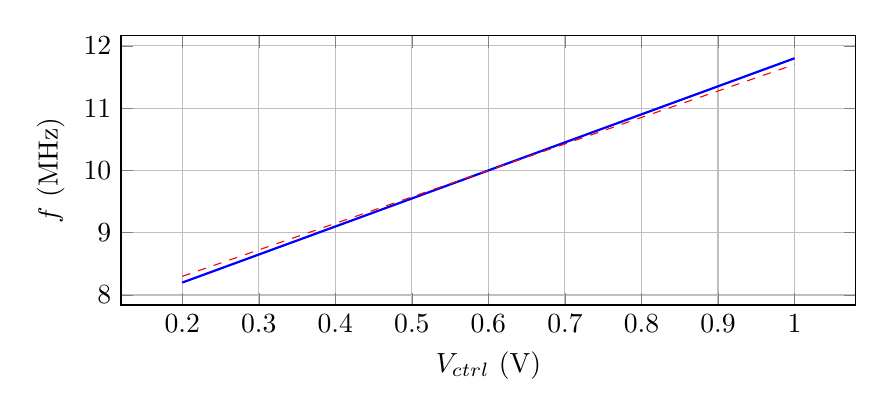
\begin{tikzpicture}
    \begin{axis}[
      width=0.9\linewidth, height=5cm,
      xlabel={$V_{ctrl}$ (V)}, ylabel={$f$ (MHz)}, grid=both]
      \addplot[blue, thick] table[row sep=\\]{
      x y \\
      0.2 8.2 \\
      0.4 9.1 \\
      0.6 10.0 \\
      0.8 10.9 \\
      1.0 11.8 \\
      };
      \addplot[red, dashed] table[row sep=\\]{
      x y \\
      0.2 8.3 \\
      1.0 11.7 \\
      };
    \end{axis}
  \end{tikzpicture}
  \caption{Example $f(V_{ctrl})$ and local linear fit around $V_{mid}$}
\end{figure}

\section{Measurement Hooks}
Expose a buffered sine output (or square via limiter), a low-noise test node for \(V_{ctrl}\) (with RC buffer), and programmable bank access. Provide on-chip dividers for low-frequency counters.

\section{Illustrative Schematic}
\begin{figure}[H]
  \centering
  \begin{circuitikz}[american]
    % Differential LC tank with cross-coupled pair
    \draw (0,0) node[ground]{} to[I, l=$I_{tail}$] (0,3)
          to[short] (-1,3) coordinate (nmid) -- (1,3) coordinate (pmid);
    % Inductor and varactor to ground (single-ended sketch for brevity)
    \draw (pmid) to[L,l=$L$] (3,3) -- (5,3)
          (3,3) to[C,l=$C(V_{ctrl})$] (3,0)
          (5,3) to[open,v^>=$V_{out}$] (5,0);
    % Cross-coupled pair symbolic
    \draw (-1,3) node[npn, xscale=1, rotate=180] (Q1) {}
          (1,3) node[npn, xscale=-1, rotate=180] (Q2) {}
          (Q1.collector) -- (pmid)
          (Q2.collector) -- (pmid)
          (Q1.emitter) -- (0,2.0)
          (Q2.emitter) -- (0,2.0)
          (Q1.base) -- (1,3) node[right] {}
          (Q2.base) -- (-1,3) node[left] {};
  \end{circuitikz}
  \caption{Complementary/cross-coupled LC VCO core with varactor tuning}
\end{figure}
\section{Design Guidelines}
\begin{itemize}
  \item Plan \(Q\) and $L$ from PN and area; back-out $C$ and varactor range with PVT margin.
  \item Use complementary cross-coupled core if close-in PN is critical; otherwise NMOS-only for lower area.
  \item Size devices for edge rate vs noise optimum; simulate jitter vs width.
  \item Filter tail current; avoid direct modulation paths into the tank.
  \item Segment coarse/fine banks for overlap; calibrate background to track drift.
  \item Harden PDN and layout for symmetry and isolation.
\end{itemize}


